Je mobiele telefoon synchroniseert zijn data met de cloud. De meeste cloud oplossingen draaien op Linux, maar wat is dat nu eigenlijk; de cloud? Letterlijk betekent cloud wolk en dat is ook waar de term vandaan komt, in tekeningen van computer netwerken wordt een totaal netwerk vaak vervangen door een wolkje. Zoals bijvoorbeeld het Internet.

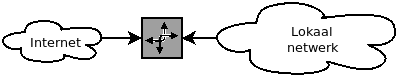
\includegraphics[width=0.99\linewidth]{Cloud_Internet.png}%

De cloud gaat dan ook over diensten die aangeboden worden in een netwerk waarbij het niet meer van belang is op welke machine de data staat, de data bevindt zich ergens in de wolk. Natuurlijk zijn er op de achtergrond fysieke machines waarop de data terecht komt en die beheert moeten worden. In dit hoofdstuk gaan we een machine inrichten met NextCloud. NextCloud is een stukje software geschreven in PHP dat je de mogelijkheid geeft om thuis een cloud systeem te bouwen. Het kan draaien op \'e\'en server met een paar gebruikers en lijkt dan ook heel erg op een NAS (Network Attached Storage) of je kan er een complete cloud dienst mee ontwikkelen dat 100K+ gebruikers ondersteunt zodat het werkt als DropBox of Google Drive. Wij zullen een simpele installatie doen op een enkele (virtuele) machine.

Een NAS gebruikt meestal FTP of SMB om bestanden te delen, Cloud systemen gebruiken het HTTP(s) protocol om via bijvoorbeeld WebDAV data te delen. Dat hoeven niet alleen bestanden te zijn, dat kan ook calender informatie (CalDAV) of adresgegevens (CardDAV) zijn. Met NextCloud zou je je telefoon dus volledig kunnen synchroniseren met je eigen server inplaats van met Google\texttrademark\ of Apple\texttrademark\.

NextCloud is een voortzetting van het ownCloud project. De ontwikkeling van ownCloud begon in 2010 en het ownCloud bedrijf ownCloud Inc. werd in 2011 opgericht door Markus Rex, Holger Dyroff and Frank Karlitschek. Het project was bedoelt als een open source vervanger van DropBox. In 2016 werd de code van ownCloud door Frank Karlitschek geforked en omgedoopt tot NextCloud. Een belangrijk deel van het ownCloud ontwikkelteam ging mee met Frank. Sinds 2017 groeit de aanhang van NextCloud, terwijl die van ownCloud daalt.
